%=======================================================
\section{Layer 2 - Monitoring}
%=======================================================
Für das Überwachen von Netzwerkverbindungen wird häufig das \textit{ICMP}\footnote{Internet Control Message Protocol zum Test der IP-Konnektivität welches mit dem Kommando \texttt{ping} verwendet wird.} Protokoll der Internetprotokollfamilie verwendet. Es genügt um festzustellen, ob ein Gerät über das Netzwerk noch erreichbar ist oder nicht. Befinden sich redundante Pfade im Netzwerk, kann eine Störung über \textit{ICMP} nicht festgestellt werden, da die \textit{ICMP-Pakete} transparent über einen redundanten Pfad geleitet werden. Die Überwachung wird mit \textit{ICMP} auf der Vermittlungs- oder Netzwerkschicht, also auf \textit{IP-Ebene} durchgeführt. In vielen Fällen werden Fehler oder Statusänderungen auf Basis von \textit{SNMP-Traps}\footnote{SNMP Traps sind Fehlermeldungen die von einer Netzwerkkomponente an einen Managementserver gesendet werden.} übermittelt. Der Status eines Netzwerkports wird beispielsweise mit einem  \textit{Link Down} oder \textit{Link Up} Trap dem Managementserver mitgeteilt.

In vielen Fällen wird entweder ein \textit{SNMP-Trap} für alle oder keinen der  Netzwerkports gesendet. Eine granulare Konfiguration für welchen der Netzwerkports Traps gesendet werden sollen fehlt häufig.

In dem folgenden Versuchsaufbau sollen drei wichtige Switch-Ports überwacht werden. Um festzustellen welche Ports für Monitoring relevant sind, verwenden wir eine benutzerdefinierte \textit{Port-Description}. Als Switch wird ein \textit{Cisco 3524XL} mit \textit{IOS 12.0(5)WC17} verwendet. \textit{OpenNMS} ist in der Version 1.8.1 auf einem \textit{Ubuntu Server 9.10} installiert. Es sind noch keine Geräte in \textit{OpenNMS} eingetragen und es findet noch keine Überwachung statt. Der Versuchsaufbau ist in der folgenden Abbildung dargestellt.

\begin{figure}[H]
	\centering
	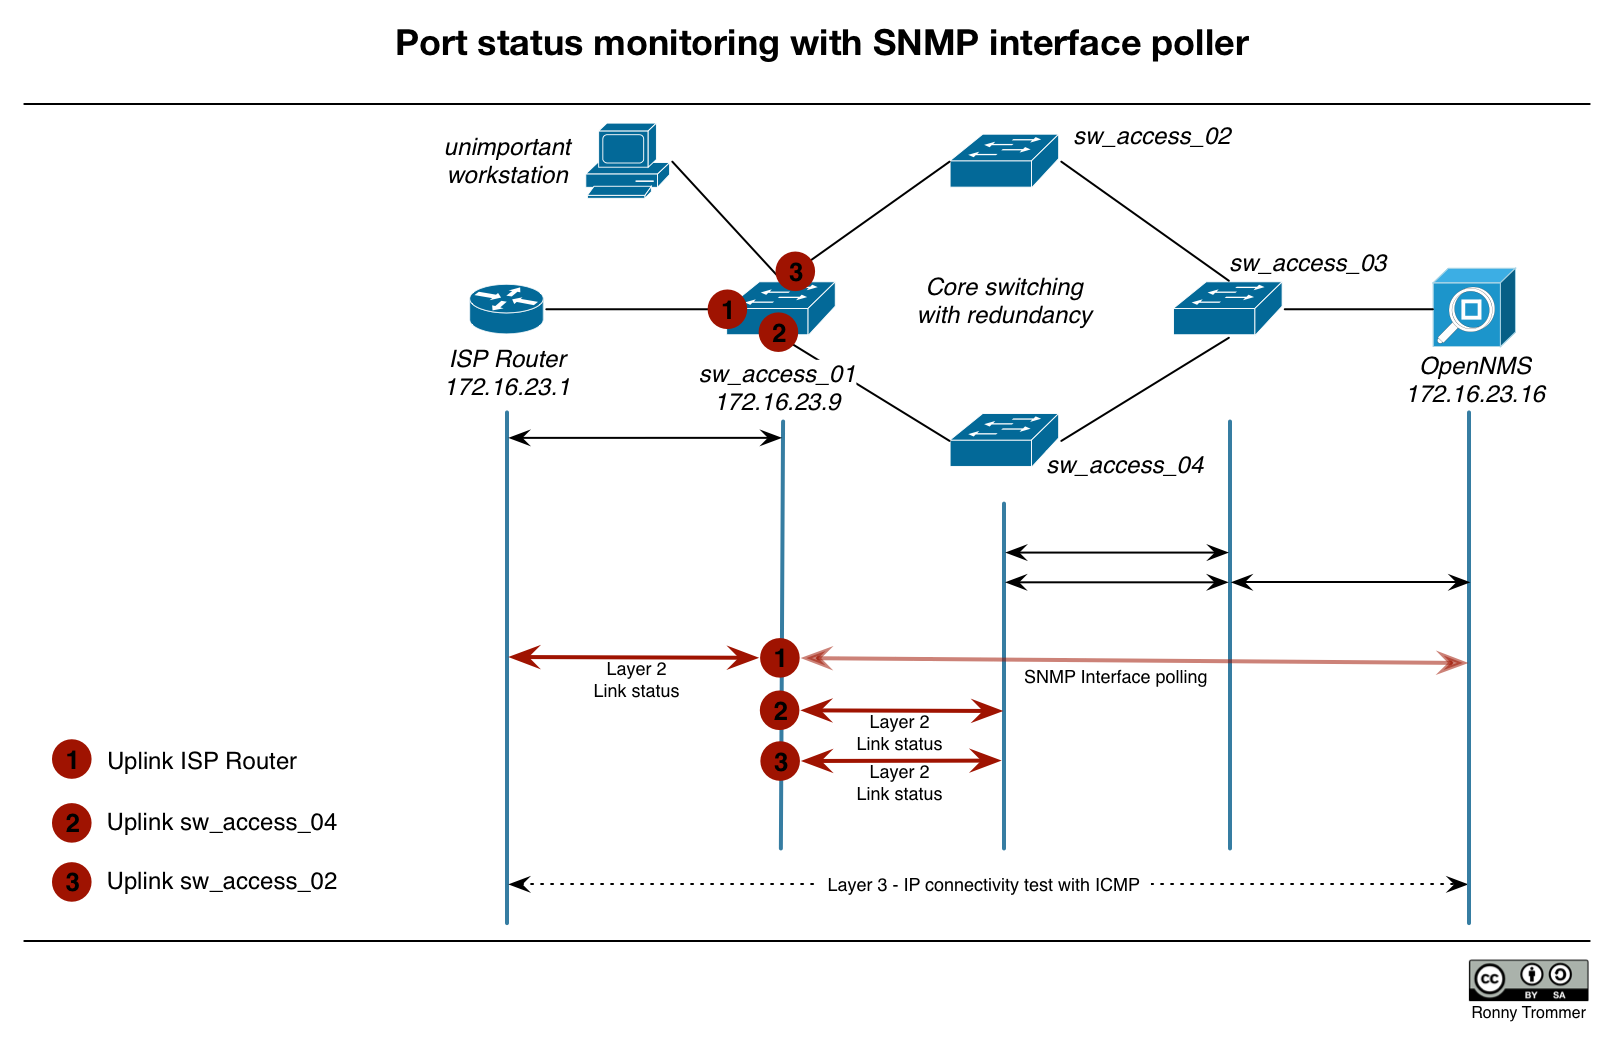
\includegraphics[width=1.0\textwidth]{images/use-cases/monitoring-layer-2/lab-plan}
	\caption{Versuchsaufbau}
	\label{pic:lab}
\end{figure}

Es sollen auf einem Switch mit der Bezeichnung \textit{sw\_access\_01}, drei wichtige Ports überwacht werden. Für die Überwachung relevant ist der Link zum \textit{ISP}\footnote{Internet Service Provider stellt den Übergabepunkt zu Internetdiensten bereit.} Router sowie auch die beiden Uplinks zum redundant ausgelegten Core. Der Port mit der Workstation interessiert uns in der Überwachung nicht und soll entsprechend ignoriert werden. In dem folgendem Versuch wird gezeigt wie \textit{SNMP} auf dem Switch eingerichtet werden kann und in \textit{OpenNMS} aufgenommen wird. Es werden lediglich Leistungsdaten von relevanten Ports aufgezeichnet. Danach wird der \textit{SNMP-Interface Poller} für die entsprechenden Ports eingerichtet.

%=======================================================
\subsection{SNMP-Ready Cisco Switch}
%=======================================================
Bevor wir überhaupt mit der Überwachung anfangen können, muss \textit{SNMP} auf den Geräten eingerichtet werden. Die Einrichtung wird detailiert auf \url{http://www.cisco.com} unter \textit{"Configuring SNMP 3"}\footnote{Configuring SNMP – \url{http://www.cisco.com/en/US/docs/ios/12_2/configfun/configuration/guide/fcf014.html}} beschrieben. Es werden hier nur die rudimentären Schritte zur Einrichtung von \textit{SNMP} beschrieben. Die grundlegende Einrichtung von Authentifizierung, Hostnamen sowie IP-Adressen ist bereits vorgenommen. Wir melden uns per \textit{Telnet} auf unserem Switch an und aktivieren \textit{SNMP} im \textit{Read-Only} Modus und setzen eine \textit{location} und einen \textit{contact}.

\lstinputlisting[caption={SNMP-Konfiguration auf Cisco Switch}
      \label{lst:cisco-snmp-config}]
  {configs/use-cases/monitoring-layer-2/cisco-snmp.cfg}

Damit ist es nun möglich vom \textit{OpenNMS-Server} \textit{SNMP} Abfragen durchzuführen. Im Anschluss werden die entsprechenden \textit{Port-Description} gesetzt.

\lstinputlisting[caption={Konfiguration der Netzwerk-Ports}
       \label{lst:cisco-port-config}]
  {configs/use-cases/monitoring-layer-2/cisco-ports.cfg}

\textbf{\textit{Hinweis:}} Es ist häufig sinnvoll, mit Hilfe von \textit{Access Listen}, Zugriffe nur von IP-Adressen des Management-Servers zu gestatten. Schauen Sie sich hier die entsprechenden \textit{ACLS} an.

Um die SNMP Konfiguration zu testen, können die gesetzten Beschreibungen mit dem Kommando

\begin{lstlisting}[numbers=none]
snmpwalk -v 2c -c notpublic 172.16.23.9 IF-MIB::ifAlias
\end{lstlisting}

vom \textit{OpenNMS-Server} abgerufen werden. Die Ausgabe sollte dann in etwa so aussehen:

\lstinputlisting[caption={\textit{SNMP walk} für die Anzeige der \textit{Port-Description}}
       \label{lst:cisco-ifalias-snmpwalk}]
  {configs/use-cases/monitoring-layer-2/cisco-ifalias-snmpwalk.txt}

Damit sind die Voraussetzungen für das Monitoring in OpenNMS erfüllt und wir können den Switch in OpenNMS für die Überwachung eintragen.

%=======================================================
\subsection{Cisco Switch Provisioning}
%=======================================================
Bevor wir Geräte eintragen, sollte die verwendete \textit{SNMP-Community} bekannt sein. Hierzu gibt es zwei Möglichkeiten, entweder die \textit{default SNMP-Community} ist in der Datei

\begin{lstlisting}[numbers=none]
$OPENNMS_HOME/etc/snmp-config.xml
\end{lstlisting}

entsprechend setzen oder die \textit{Community} wird für die einzelne IP-Adresse oder einen IP-Bereich über die Web-Oberfläche gesetzt. Um die \textit{SNMP-Community} für unseren Switch mit der IP 172.16.23.9 zu setzen, wird das Formular in der Web-Oberfläche wie folgt ausgefüllt.

\begin{lstlisting}[numbers=none]
Admin --> Configure SNMP Community Names by IP
\end{lstlisting}

\begin{figure}[H]
	\centering
	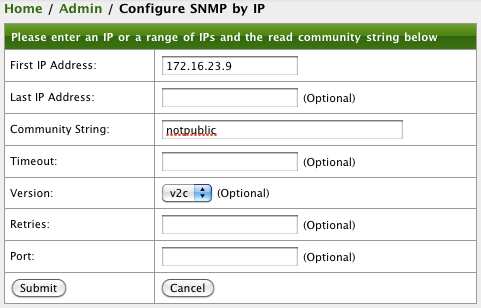
\includegraphics[width=1.0\textwidth]{images/use-cases/monitoring-layer-2/configure-snmp-by-ip}
	\caption{SNMP Community für IP-Adressen konfigurieren}
	\label{pic:configure-snmp-by-ip}
\end{figure}

Im nächsten Schritt wird der Switch über das \textit{Provisioning} von \textit{OpenNMS} aufgenommen. Wir erzeugen eine neue \textit{Requisition Group} über 

\begin{lstlisting}[numbers=none]
Admin --> Manage Provisioning Groups --> Add New Group
\end{lstlisting}

mit der Bezeichnung \textit{OpenNMS Lab}. Wir erstellen eine \textit{Policy}\footnote{\textit{Policies} beschreiben Richtlinien für das Monitoring in \textit{OpenNMS} und werden während des Import in die \textit{OpenNMS-Datenbank} angewendet.} die nur Leistungsdaten von relevanten und aktiven Ports aufzeichnet. Zusätzlich soll nur \textit{ICMP} und \textit{SNMP} für den Switch überwacht werden. Die \textit{Policy} sieht dazu wie folgt aus:

\begin{figure}[H]
	\centering
	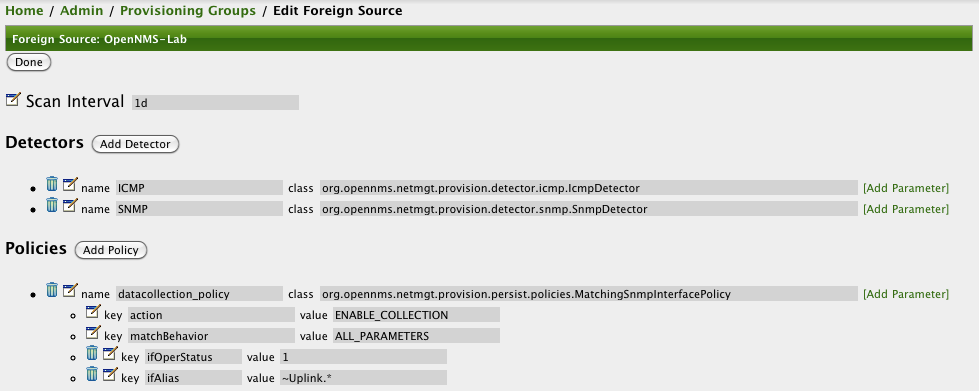
\includegraphics[width=1.0\textwidth]{images/use-cases/monitoring-layer-2/requisition-policy}
	\caption{Richtlinie für den Import des \textit{Cisco} Switch}
	\label{pic:requisition-policy}
\end{figure}

Alle Detektoren ausser \textit{ICMP} und \textit{SNMP} wurden entfernt. Zusätzlich wurde eine \textit{datacollection\_policy} angelegt, die nur Leistungsdaten von Ports aufzeichnet, welche aktiv sind und\footnote{Die Verknüpfung stammt aus dem Konfigurationsschlüssel \textit{matchBehavior}, \textit{oder=ANY\_PARAMETER}, \textit{Negation=NON\_PARAMETERS}} eine Port-Beschreibung\footnote{In der \textit{SNMP MIB II} ist \textit{ifDescr} die Interface-Bezeichnung \textit{(FastEthernet 0/1)} und der \textit{ifAlias} die Port Beschreibung} mit \textit{Uplink} beginnend besitzen. Die Geräte in der \textit{Requisition Group} wird täglich\footnote{Definiert über den Standardparameter \textit{Scan Interval 1d}} einmal synchronisiert. Der Switch wird nun unter 

\begin{lstlisting}[numbers=none]
Requisition (Provisioning Group): EDIT --> Add Node
\end{lstlisting}

eingetragen und synchronisiert.

\begin{figure}[H]
	\centering
	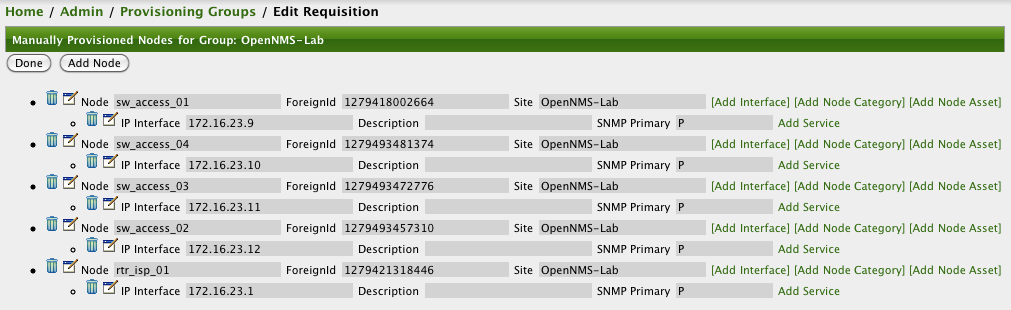
\includegraphics[width=1.0\textwidth]{images/use-cases/monitoring-layer-2/requisition-import}
	\caption{Import der \textit{Requisition Group} in \textit{OpenNMS}}
	\label{pic:requisition-import}
\end{figure}

Die Konfiguration wird bestätigt, über die Schaltfläche \textit{Synchronize} importiert und im Monitoring bereitgestellt. Nach dem Import stellt sich der Switch in OpenNMS wie folgt dar:

\begin{figure}[H]
	\centering
	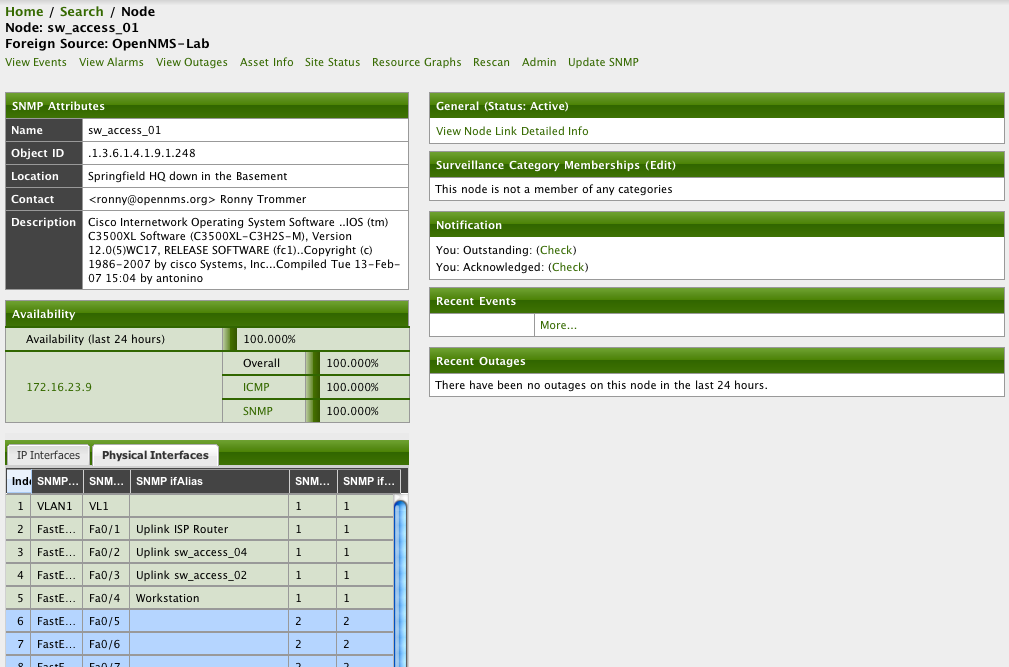
\includegraphics[width=1.0\textwidth]{images/use-cases/monitoring-layer-2/node-page}
	\caption{\textit{Node Page} des Cisco-Switch nach dem Import in \textit{OpenNMS}}
	\label{pic:node-page}
\end{figure}

Zur besseren Darstellung wurden die Spalten mit der Interface-Geschwindigkeit und IP-Adresse ausgeblendet und der \textit{Port-Status} hinzugefügt. Die grün hinterlegten Ports sind aktiv. Die blau hinterlegten Ports sind administrativ deaktiviert. Der Switch wird nun täglich  mit den entsprechenden Port-Beschreibungen in OpenNMS synchronisiert und die entsprechenden Informationen im Monitoring bereitgestellt. Es werden zusätzlich nur Leistungsdaten von Ports mit der Beschreibung \textit{Uplink} aufgezeichnet.

\begin{figure}[H]
	\centering
	\includegraphics[width=1.0\textwidth]{images/use-cases/monitoring-layer-2/uplink-datacollection}
	\caption{Leistungsdaten werden nur von Ports mit der Beschreibung \textit{Uplink} gesammelt.}
	\label{pic:uplink-datacollection}
\end{figure}

%=======================================================
\subsection{Port Status kontrollieren}
%=======================================================
Zu Begin muss der dazu verwendete \textit{SNMP Interface Poller} aktiviert werden. In der Datei

\begin{lstlisting}[numbers=none]
$OPENNMS_HOME/etc/service-configuration.xml
\end{lstlisting}

wird dazu der entsprechende Dienst auskommentiert.

\lstinputlisting[language=XML, caption={Der \textit{SNMP Interface Poller} ist nach der Installation von \textit{OpenNMS} einkommentiert.}
       \label{lst:opennms-service-ifpoller}]
  {configs/use-cases/monitoring-layer-2/opennms-service-config.xml}

Im nächsten Schritt wird ein \emph{Interface Polling Package} angelegt. In diesem wird festgelegt, welche Ports zu überwachen sind.

\begin{lstlisting}[numbers=none]
vi $OPENNMS_HOME/etc/snmp-interface-poller-configuration.xml
\end{lstlisting}

Die package-Beschreibung wird wie folgt aufgebaut:

\lstinputlisting[language=XML, caption={\textit{Polling-Package} für den \textit{SNMP-Interface Poller}}
       \label{lst:opennms-ifpoller-package}]
  {configs/use-cases/monitoring-layer-2/snmp-interface-poller-package-config.xml}

Damit nur Ports mit der Beschreibung \textit{Uplink} überwacht werden, wird ein Filterkritierum angegeben. Dieses lässt sich logisch mit weiteren Kriterien mit \textit{AND} und \textit{OR} verknüpfen. Mit \textit{snmpifalias like 'Uplink\%'} wird der entsprechende \textit{Alias} aus der Datenbank ausgelesen und überwacht. Der Port Status wird alle 5 Minuten getestet und aktualisiert. Es können als Bedingung alle Felder aus der Tabelle \textit{snmpinterface} verwendet werden. In der Version 1.8.1 sind folgende Spalten verwendbar:

\pagebreak

\begin{longtable}{|p{3.5cm}|p{11cm}|}
  % Kopf auf erste Seite
  \hline
    \rowcolor{light_gray}[5.8pt]
 	 Bezeichnung	&	Beschreibung \\
	 \hline
	 \endfirsthead
	 %Kopf auf weiteren Seiten
	 \hline \multicolumn{2}{|c|}{(Fortsetzung)}\\
	 \hline
	 \rowcolor{light_gray}[5.8pt]
	 Bezeichnung	&	Beschreibung \\
	 \hline
	 \endhead
	 \hline
	 \multicolumn{2}{|c|}{(Tabelle wird auf der nächsten Seite fortgesetzt)}
  \endfoot
  \hline
	\caption{Verwendbare Attribute der SNMP interface table}
  \endlastfoot
	\hline
  	nodeid    &    Eindeutige ID für den Knoten in OpenNMS. \\
  	\hline
  	ipaddr    &    RFC-1213-MIB: The media-dependent physical address. Setting this object to a null string (one of zero length) has the effect of invaliding the corresponding entry in the atTable object.  That is, it effectively dissasociates the interface identified with said entry from the mapping identified with said entry.  It is an implementation-specific matter as to whether the agent removes an invalidated entry from the table. Accordingly, management stations must be prepared to receive tabular information from agents that corresponds to entries not currently in use. Proper interpretation of such entries requires examination of the relevant atPhysAddress object. \\
  	\hline
  	snmpipadentnetmask    &    RFC1213-MIB: The NetworkAddress (e.g., the IP address) corresponding to the media-dependent `physical' address. \\
  	\hline
  	snmpphysaddr    &    RFC-1213-MIB: The interface's address at the protocol layer immediately `below' the network layer in the protocol stack.  For interfaces which do not have such an address (e.g., a serial line), this object should contain an octet string of zero length. \\
  	\hline
  	snmpifdescr    &    RFC-1213-MIB: A textual string containing information about the interface.  This string should include the name of the manufacturer, the product name and the version of the hardware interface. \\
  	\hline
  	snmpiftype    &    RFC-1213-MIB (Nur ein Auszug): Interface type
other(1), ethernetCsmacd(6), basicISDN(20), primaryISDN(21), propPointToPointSerial(22), ppp(23),softwareLoopback(24), frameRelay(32), atm(37), aal5(49), isdn(63), adsl(94), sdsl(96), vdsl(97), pppMultilinkBundle(108), atmVirtual(149),mplsTunnel(150), mpls166), adsl2(230), adsl2plus(238)
RFC-1213-MIB: The type of interface, distinguished according to the physical/link protocol(s) immediately `below' the network layer in the protocol stack. \\
    \hline
    snmpifname    &    Bei Cisco Kurzbezeichnung Fa/0/2 \\
    \hline
    snmpifspeed    &    RFC-1213-MIB:  An estimate of the interface's current bandwidth in bits per second.  For interfaces which do not vary in bandwidth or for those where no accurate estimation can be made, this object should contain the nominal bandwidth. \\
    \hline
    snmpifadmin    &    Administrativer Status: up(1), down(2), testing(3)
RFC-1213-MIB: The desired state of the interface.  The testing(3) state indicates that no operational packets can be passed. \\
    \hline
    snmpifoperstatus    &    Operativer Status: up(1), down(2), unknown(4), dormant(5), notPresent(6), lowerLayerDown(7)
RFC-1213-MIB: The current operational state of the interface. The testing(3) state indicates that no operational packets can be passed. \\
    \hline
    snmpifalias    &    Eigene Port Beschreibung \\
    \hline
    snmpcollect    &    (N) Not Collect oder (C) Collect.Gibt an ob Leistungsdaten aufgezeichnet werden sollen oder nicht.
    \label{tbl:snmpifattrib}
\end{longtable}

Die vollständige Konfigurationsdatei wird im folgenden komplett dargestellt.

\lstinputlisting[language=XML, caption={SNMP Interface Poller konfiguration.}
       \label{lst:opennms-ifpoller-configuration}]
  {configs/use-cases/monitoring-layer-2/snmp-interface-poller-config.xml}

Damit die Einstellung wirksam werden, muss OpenNMS neu gestartet werden.

\begin{lstlisting}[numbers=none]
service opennms restart
\end{lstlisting}

%=======================================================
\subsection{Funktionstest}
%=======================================================
Im nächsten Schritt prüfen wir das Verhalten von OpenNMS wenn verschiedene Ports den Status ändern. Dazu werden zwei Testszenarien geprüft:

\begin{enumerate}
  \item{Ein Uplink Port und der Workstation Port werden abgezogen und ein Ausfall simuliert. Es sollte nur ein Port Down Event auf dem Uplink Port erzeugt werden.}
  \item{Ein Uplink Port und der Workstation Port werden administrativ down gesetzt. Zusätzlich simulieren wir eine echte Störung auf dem Uplink zum ISP-Router.}
\end{enumerate}

In der Ausgangssituation läuft alles wie gewünscht. Alle Ports sind aktiv und funktionsbereit.

\begin{figure}[H]
	\centering
	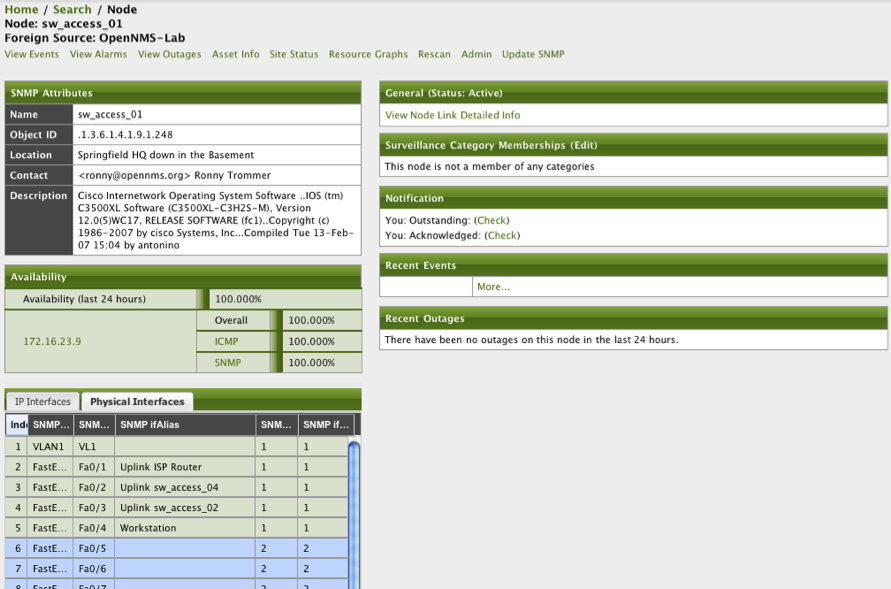
\includegraphics[width=1.0\textwidth]{images/use-cases/monitoring-layer-2/node-page-snmpifpoller}
	\caption{Node page mit Port status für \emph{Physical Interfaces}.}
	\label{pic:node-page-snmpifpoller}
\end{figure}

%=======================================================
\subsubsection{Szenario 1: Port Störungen}
%=======================================================
Die Ports \emph{Fa0/3} und \emph{Fa0/4} wurden abgezogen und simulieren einen Ausfall. Wir sehen, dass der Portstatus nur für den Port \emph{Fa0/3} aktualisiert wurde.

\begin{figure}[H]
	\centering
	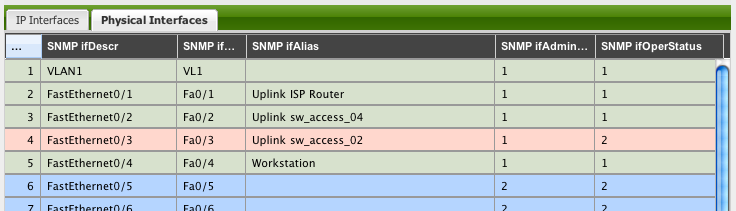
\includegraphics[width=1.0\textwidth]{images/use-cases/monitoring-layer-2/port-outage}
	\caption{Anzeige Port Störung eines \emph{Physical Interfaces}.}
	\label{pic:port-outage-snmpifpoller}
\end{figure}

OpenNMS erzeugt zusätzlich ein entsprechendes Event und protokolliert damit das Ereignis.

\begin{figure}[H]
	\centering
	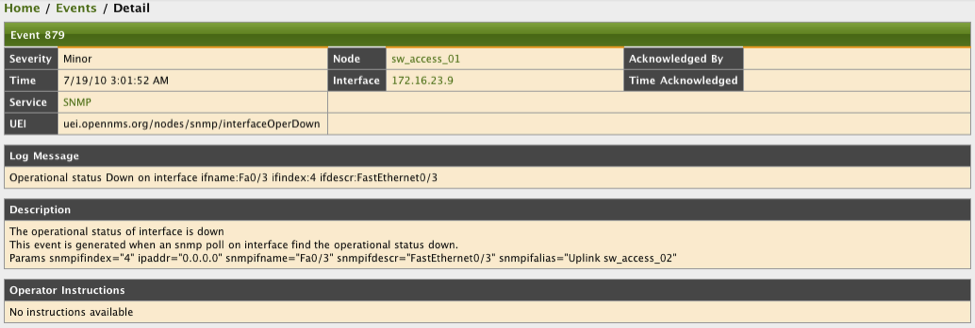
\includegraphics[width=1.0\textwidth]{images/use-cases/monitoring-layer-2/port-down-event}
	\caption{\emph{Event} bei Port-Störung.}
	\label{pic:port-down-event}
\end{figure}

Der Status des Ports \emph{Fa0/4} wird nicht durch den \emph{SNMP-Interface Poller} aktualisiert. Es wurde ja explizit angegeben, dass nur \emph{Uplink} Ports überwacht werden. Erst bei einer neuen Synchronisation der kompletten \emph{Provisioning Group} wird auch der entsprechende Port-Status der Workstation wieder mit übernommen. Das Interval beträgt einen Tag. Wir synchronisieren manuell und der entsprechende Port Status wird wie folgt angzeigt.

\begin{figure}[H]
	\centering
	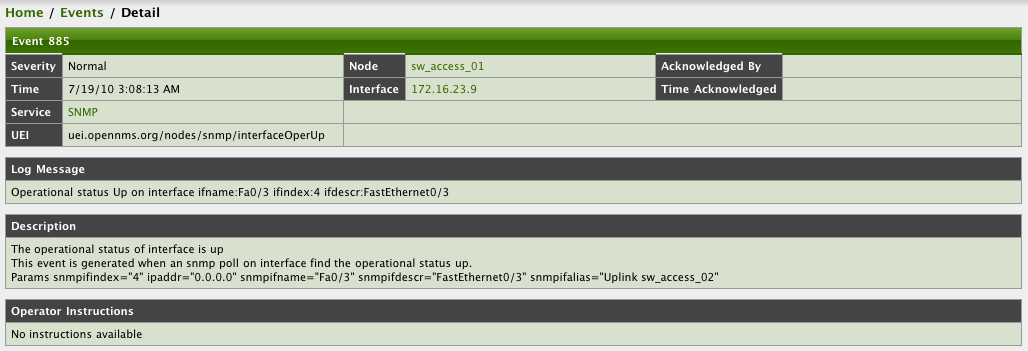
\includegraphics[width=1.0\textwidth]{images/use-cases/monitoring-layer-2/port-up-event}
	\caption{\emph{Event} beim auflösen der Port-Störung.}
	\label{pic:port-up-event}
\end{figure}

Damit ist der erste Testfall erfolgreich abgeschlossen. Im zweiten Testfall prüfen wir, ob der Administrative Status korrekt überwacht wird.

%=======================================================
\subsubsection{Szenario 2: Störung und administrativ deaktiviert}
%=======================================================
Wir gehen wie gehabt von einem voll funktionsfähigem Netzwerk aus. Alle Ports sind aktiv und funktionsbereit. Es werden nun wiederum zwei Ports manuell deaktiviert8. Der Status sieht nun wie folgt aus.

\begin{figure}[H]
	\centering
	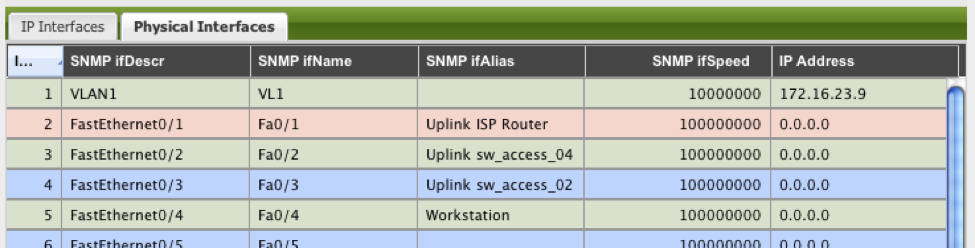
\includegraphics[width=1.0\textwidth]{images/use-cases/monitoring-layer-2/port-admin-down}
	\caption{Interface status nach administrativen deaktivieren des Ports.}
	\label{pic:port-admin-down}
\end{figure}

Wir erhalten zwei unterschiedliche Meldungen und zwar über den Port \emph{Fa0/1} sowie \emph{Fa0/3}. Der Port \emph{Fa0/4} für die Workstation wird komplett ignoriert. Für den administrativen Status wird ein eigenes Event \emph{interfaceAdminDown} erzeugt.

\begin{figure}[H]
	\centering
	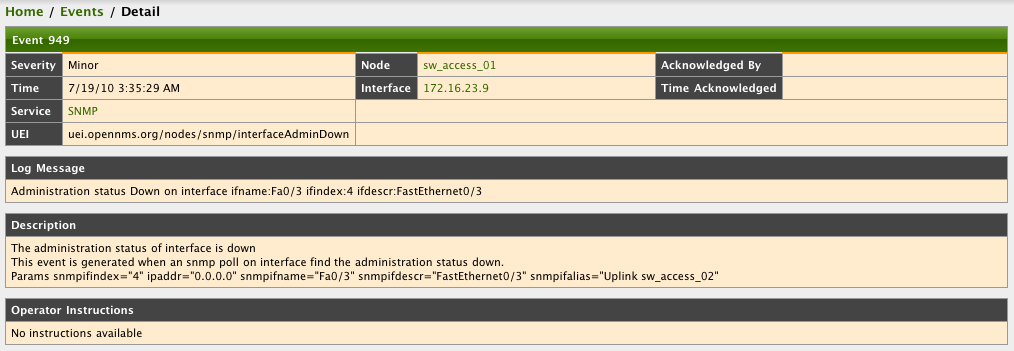
\includegraphics[width=1.0\textwidth]{images/use-cases/monitoring-layer-2/port-admin-down-event}
	\caption{\emph{Event} nach dem administrativen deaktivieren des Ports.}
	\label{pic:port-admin-down-event}
\end{figure}

Bei einer echten Störung wird ein Event \emph{interfaceOperDown} generiert. Damit ist der Funktionstest abgeschlossen und auf die entsprechenden Events können verschiedene Benachrichtigungen eingerichtet werden. Für die Benachrichtigung stehen die folgenden Events zur Verfügung

\begin{itemize}
  \item{Snmp Interface Admin Status Down}
  \item{Snmp Interface Admin Status Up}
  \item{Snmp Interface Oper Status Down}
  \item{Snmp Interface Oper Status Up}
\end{itemize}

Damit sollte einer Port Status Überwachung in OpenNMS nichts mehr im Wege stehen.